\section{RGB Rendering of COGITAO} \label{appendix:rgb_cogitao}

\begin{figure}[!htbp]
    \centering
    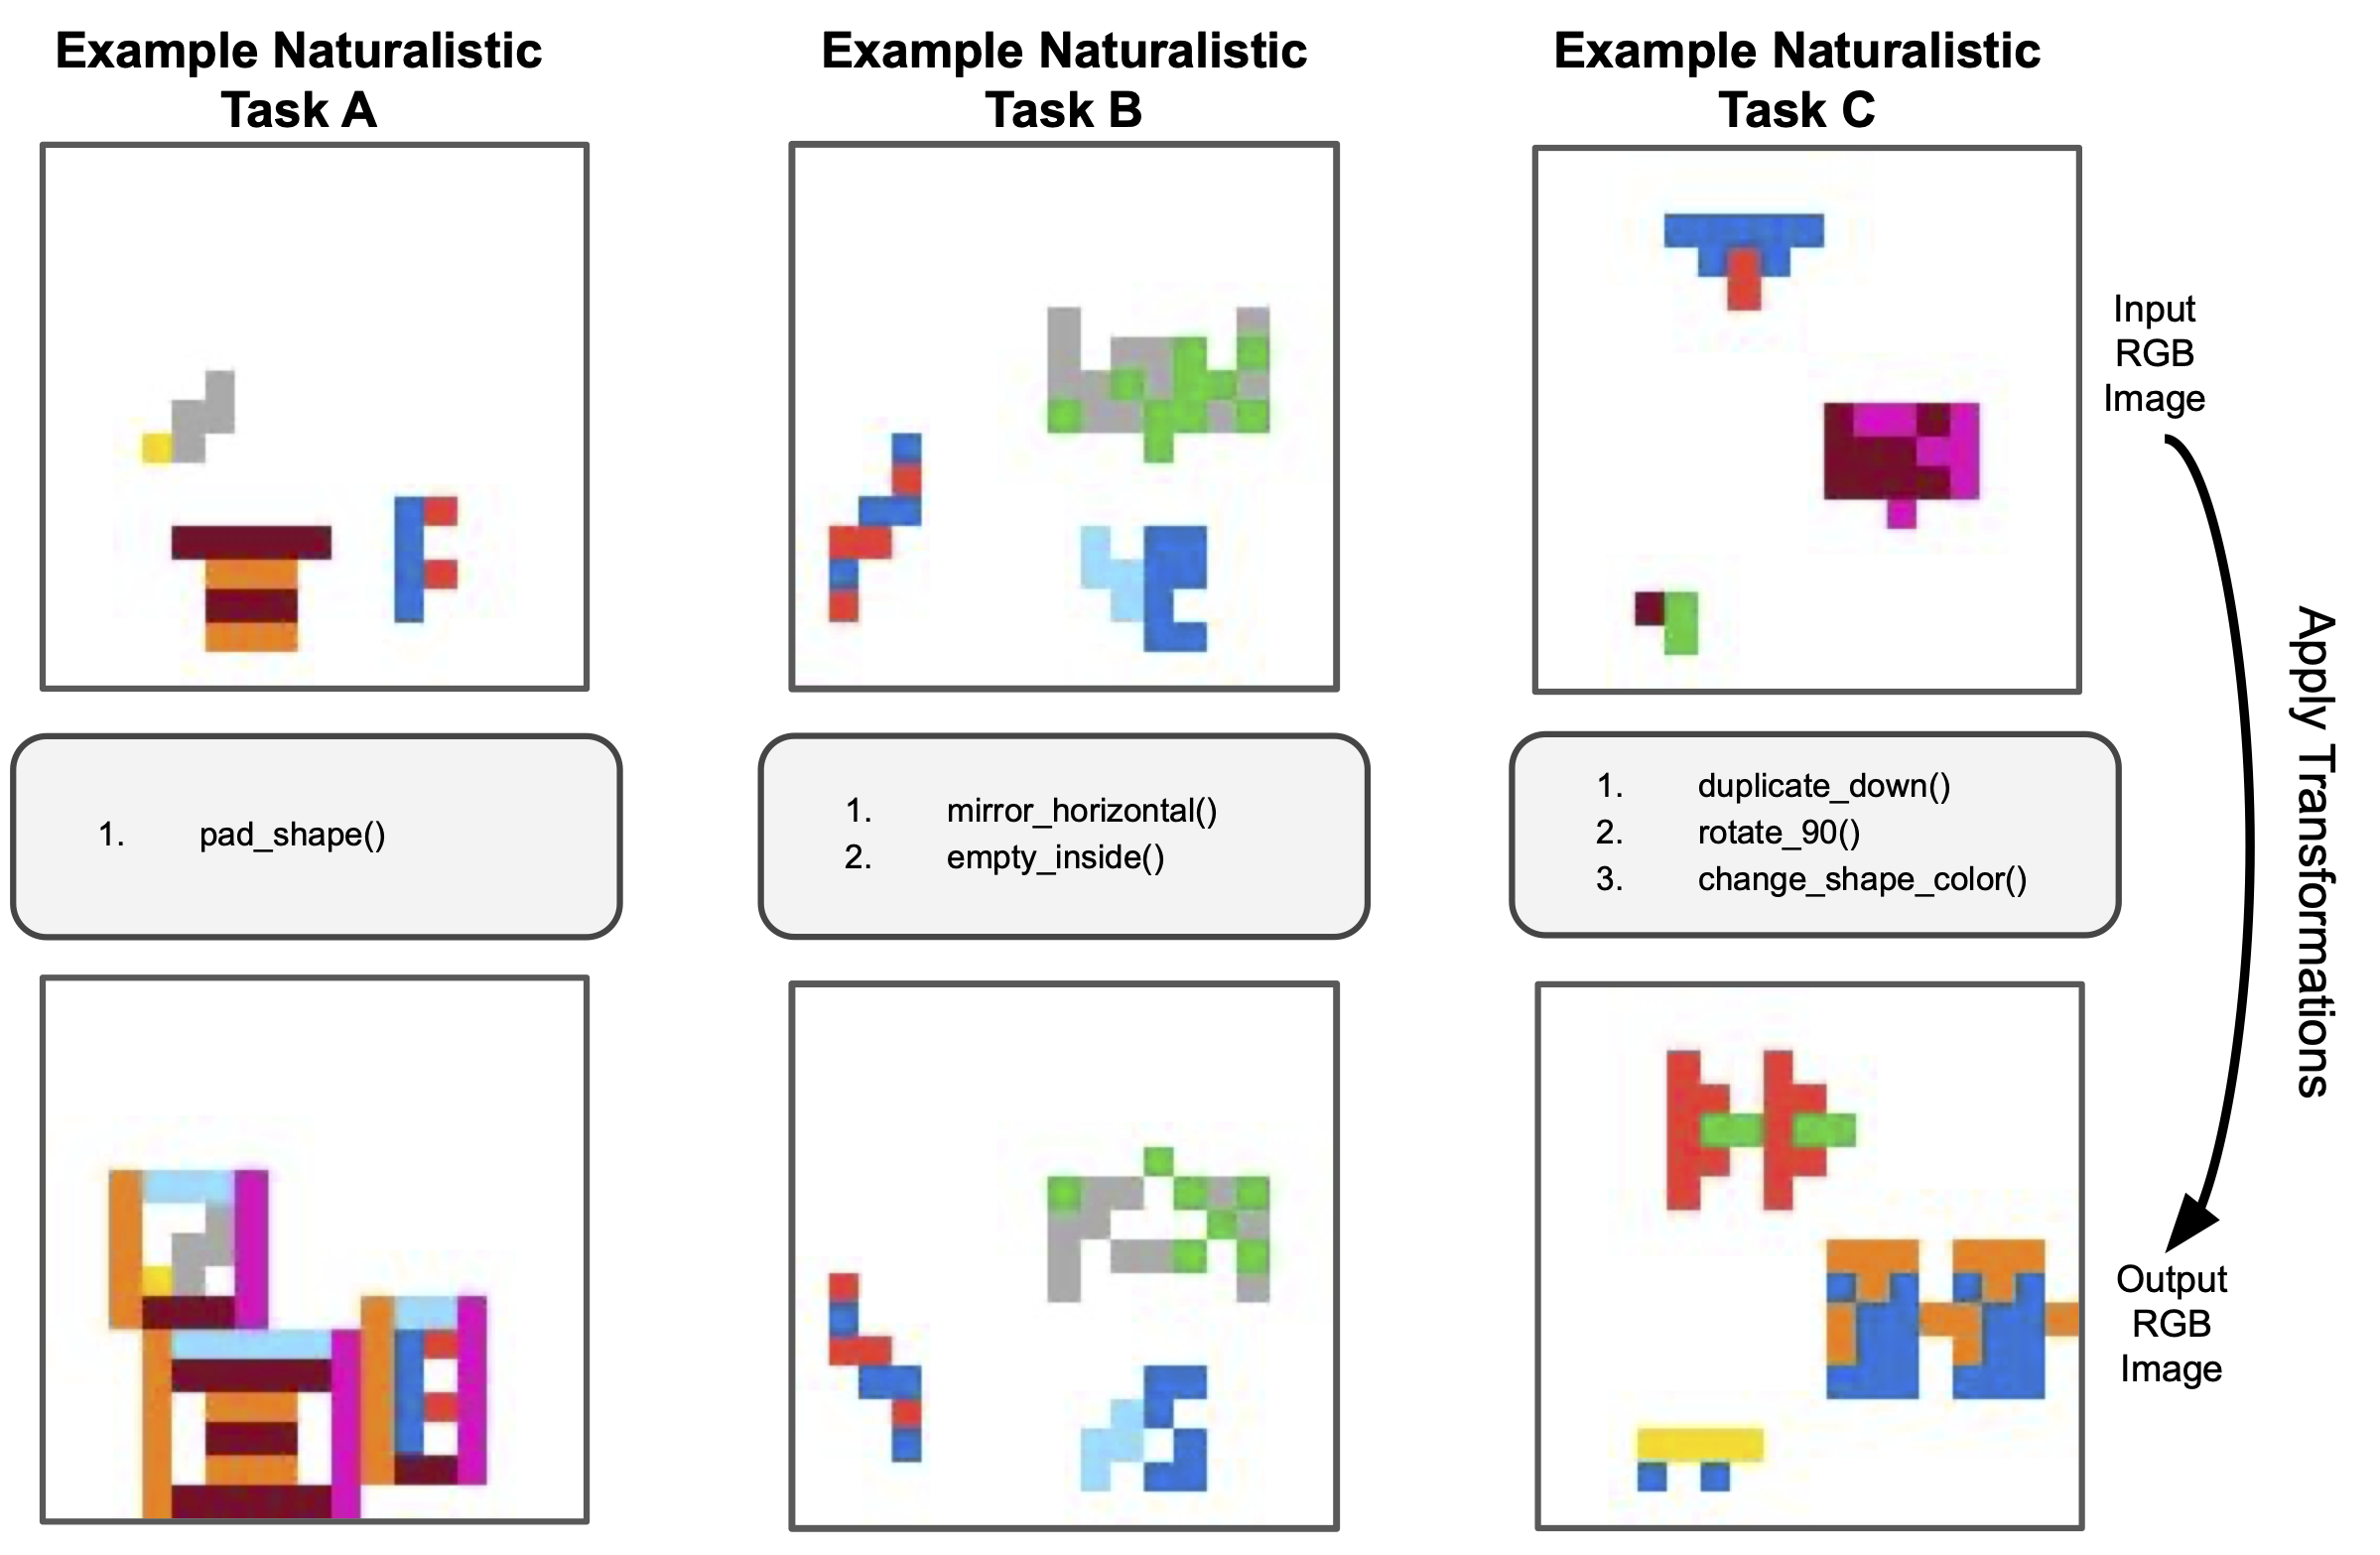
\includegraphics[width=1\columnwidth]{Figures/naturalistic_Cogitao.png}
    \caption{Set of input-output pair examples from our RGB rendering of \generatorName\, with input \textit{images} on top rows, and corresponding output \textit{images} (after transforming input) on the bottom rows. The images are 128x128x3, saved as .jpeg. Gray borders are added for visualization purposes only - they are not present on the images. Note: Objects are purposely blurry to outline their RGB nature - crisper rendering are straightforward.}
    \label{fig:naturalistic_COGITAO}
\end{figure}

To assess how compositional generalization persists beyond synthetic grids, we introduce \generatorName-RGB, a rendering of the benchmark in standard RGB images. Each sample is a 128 $\times$ 128 RGB image (with configurable resolution) in which the discrete grid visualization is removed and objects are drawn on a plain white (or black) background. We convert the benchmark datasets presented in \ref{sec:experiment_details} to this format, excluding G1-2 and G1-5 where variable grid sizes are essential; G1-1, G1-3, and G1-4 translate directly.
All 28 transformations from \S\ref{appendix:COGITAO_transformations} remain fully applicable, but models must now infer object location and scale without explicit grid cues, increasing perceptual difficulty. Generation and train/test splits follow the original procedure. \generatorName-RGB thus bridges abstract grid worlds and natural image statistics, enabling researchers to test whether compositional and systematic generalization tested in the grid setting carries over to more realistic visual conditions.

